%% (Master) Thesis template
% Template version used: v1.4
%
% Largely adapted from Adrian Nievergelt's template for the ADPS
% (lecture notes) project.



%% We use the memoir class because it offers a many easy to use features.
\documentclass[11pt,a4paper,table,hidelinks]{memoir}  % Remove "hidelinks" for red boxes around hyperlinks

%% Packages
%% ========

%% LaTeX Font encoding -- DO NOT CHANGE
\usepackage[OT1]{fontenc}

%% Babel provides support for languages.  'english' uses British
%% English hyphenation and text snippets like "Figure" and
%% "Theorem". Use the option 'ngerman' if your document is in German.
%% Use 'american' for American English.  Note that if you change this,
%% the next LaTeX run may show spurious errors.  Simply run it again.
%% If they persist, remove the .aux file and try again.
\usepackage[english]{babel}

%% Input encoding 'utf8'. In some cases you might need 'utf8x' for
%% extra symbols. Not all editors, especially on Windows, are UTF-8
%% capable, so you may want to use 'latin1' instead.
\usepackage[utf8]{inputenc}

%% This changes default fonts for both text and math mode to use Herman Zapfs
%% excellent Palatino font.  Do not change this.
%\usepackage[sc]{mathpazo}

%% The AMS-LaTeX extensions for mathematical typesetting.  Do not
%% remove.
\usepackage{amsmath,amssymb,amsfonts,mathrsfs}

%% NTheorem is a reimplementation of the AMS Theorem package. This
%% will allow us to typeset theorems like examples, proofs and
%% similar.  Do not remove.
%% NOTE: Must be loaded AFTER amsmath, or the \qed placement will
%% break
\usepackage[amsmath,thmmarks]{ntheorem}

%% LaTeX' own graphics handling
\usepackage{graphicx}

%% We unfortunately need this for the Rules chapter.  Remove it
%% afterwards; or at least NEVER use its underlining features.
\usepackage{soul}

%% This allows you to add .pdf files. It is used to add the
%% declaration of originality.
\usepackage{pdfpages}

\newenvironment{conditions}
  {\par\vspace{\abovedisplayskip}\noindent\begin{tabular}{>{$}l<{$} @{${}={}$} l}}
  {\end{tabular}\par\vspace{\belowdisplayskip}}

%% Some more packages that you may want to use.  Have a look at the
%% file, and consult the package docs for each.
%% See the TeXed file for more explanations

%% [OPT] Multi-rowed cells in tabulars
%\usepackage{multirow}

%% [REC] Intelligent cross reference package. This allows for nice
%% combined references that include the reference and a hint to where
%% to look for it.
\usepackage{varioref}

%% [OPT] Easily changeable quotes with \enquote{Text}
%\usepackage[german=swiss]{csquotes}

%% [REC] Format dates and time depending on locale
\let\ordinal\relax %% prevent warning
\usepackage{datetime}

%% [OPT] Provides a \cancel{} command to stroke through mathematics.
%\usepackage{cancel}

%% [NEED] This allows for additional typesetting tools in mathmode.
%% See its excellent documentation.
\usepackage{mathtools}

%% [NEED] Conditional commands
\usepackage{ifthen}

%% [OPT] Manual large braces or other delimiters.
%\usepackage{bigdelim, bigstrut}

%% [REC] Alternate vector arrows. Use the command \vv{} to get scaled
%% vector arrows.
\usepackage[h]{esvect}

%% [NEED] Some extensions to tabulars and array environments.
\usepackage{array}

%% [OPT] Postscript support via pstricks graphics package. Very
%% diverse applications.
%\usepackage{pstricks,pst-all}

%% [?] This seems to allow us to define some additional counters.
%\usepackage{etex}

%% [ADV] XY-Pic to typeset some matrix-style graphics
%\usepackage[all]{xy}

%% [OPT] This is needed to generate an index at the end of the
%% document.
%\usepackage{makeidx}

%% [OPT] Fancy package for source code listings.  The template text
%% needs it for some LaTeX snippets; remove/adapt the \lstset when you
%% remove the template content.
\usepackage{listings}
% \lstset{language=TeX,basicstyle={\normalfont\ttfamily}}

%% [REC] Fancy character protrusion.  Must be loaded after all fonts.
%\usepackage[activate]{pdfcprot}

%% [REC] Nicer tables.  Read the excellent documentation.
\usepackage{booktabs}

%% [OPT] Package for adding TODOs.
\usepackage{todonotes}

%% [OPT] Package to define and use acronyms
\usepackage[nolist,nohyperlinks,smaller]{acronym}

\usepackage{caption}
\usepackage{subcaption}
\expandafter\def\csname ver@subfig.sty\endcsname{}
 

%% Our layout configuration.  DO NOT CHANGE.
%% Memoir layout setup

%% NOTE: You are strongly advised not to change any of them unless you
%% know what you are doing.  These settings strongly interact in the
%% final look of the document.

% Dependencies
%\usepackage{ETHlogo}

% use helvetica as default font:
\usepackage[scaled]{helvet}
%\renewcommand\familydefault{\sfdefault} 

% Turn extra space before chapter headings off.
\setlength{\beforechapskip}{0pt}

\nonzeroparskip
\parindent=0pt
\defaultlists

% Chapter style redefinition
\makeatletter

\makepagestyle{headerWPageNr}% Create headerWPageNr style
\if@twoside
  \copypagestyle{headerWPageNr}{Ruled}
  \copypagestyle{chapter}{Ruled}
\else
  \copypagestyle{headerWPageNr}{ruled}
  \copypagestyle{chapter}{ruled}
\fi
% chapter pages have no header and center page number in footer:
\makeoddhead{chapter}{}{}{}
\makeevenhead{chapter}{}{}{}
\makeoddfoot{chapter}{}{\thepage}{}
\makeevenfoot{chapter}{}{\thepage}{}
\makeheadrule{chapter}{\textwidth}{0pt}

% all other pages have page number and chapter or section name in header without footer:
\makeoddhead{headerWPageNr}{\rightmark}{}{\thepage}
\makeevenhead{headerWPageNr}{\thepage}{}{\leftmark}
\makeoddfoot{headerWPageNr}{}{}{}
\makeevenfoot{headerWPageNr}{}{}{}
\pagestyle{headerWPageNr}% Set page style to headerWPageNr


\makechapterstyle{bianchimod}{%
  \copypagestyle{abstract}{empty}
  \copypagestyle{acknowledgement}{empty}
  \chapterstyle{default}
  \renewcommand*{\chapnamefont}{\normalfont\Large\sffamily}
  \renewcommand*{\chapnumfont}{\normalfont\Large\sffamily}
  \renewcommand*{\printchaptername}{%
    \chapnamefont\centering\@chapapp}
  \renewcommand*{\printchapternum}{\chapnumfont {\thechapter}}
  \renewcommand*{\chaptitlefont}{\normalfont\huge\sffamily}
  \renewcommand*{\printchaptertitle}[1]{%
    \hrule\vskip\onelineskip \centering \chaptitlefont\textbf{\vphantom{gyM}##1}\par}
  \renewcommand*{\afterchaptertitle}{\vskip\onelineskip \hrule\vskip
    \afterchapskip}
  \renewcommand*{\printchapternonum}{%
    \vphantom{\chapnumfont {9}}\afterchapternum}}
  
\makechapterstyle{bianchimod2}{%
  \renewenvironment{abstract}{\chapter*{\abstractname}}{}
  \newenvironment{acknowledgement}{\chapter*{Acknowledgement}}{}
  \chapterstyle{default}
  \definecolor{ChapGrey}{rgb}{0.6,0.6,0.6}
  \newcommand{\LargeFont}{% Needs a ’stretchable’ font
  	\usefont{\encodingdefault}{\sfdefault}{b}{n}%
    \fontsize{100}{0}\selectfont\color{ChapGrey}}
  \renewcommand*{\chapnumfont}{\LargeFont}
  \renewcommand*{\printchaptername}{\raggedleft}
  \renewcommand*{\printchapternum}{\chapnumfont {\thechapter}}
  \renewcommand*{\chaptitlefont}{\normalfont\Huge\sffamily\color{black}}
  \renewcommand*{\printchaptertitle}[1]{%
    \raggedleft \chaptitlefont\textbf{\vphantom{gyM}##1}\par}}

% Use the newly defined style
\chapterstyle{bianchimod2}

\setsecheadstyle{\Large\bfseries\sffamily}
\setsubsecheadstyle{\large\bfseries\sffamily}
\setsubsubsecheadstyle{\bfseries\sffamily}
\setparaheadstyle{\normalsize\bfseries\sffamily}
\setsubparaheadstyle{\normalsize\itshape\sffamily}
\setsubparaindent{0pt}

% Set captions to a more separated style for clearness
\captionnamefont{\sffamily\bfseries\footnotesize}
\captiontitlefont{\sffamily\footnotesize}
\setlength{\intextsep}{16pt}
\setlength{\belowcaptionskip}{1pt}

% Set section and TOC numbering depth to subsection
\setsecnumdepth{subsection}
\settocdepth{subsection}

% definitions for titlepage
\def\@advisor{}
\newcommand{\advisor}[1]{\def\@advisor{#1}}
\def\@supervisor{}
\newcommand{\supervisor}[1]{\def\@supervisor{#1}}
\def\@group{}
\newcommand{\group}[1]{\def\@group{#1}}
\def\@institute{}
\newcommand{\institute}[1]{\def\@institute{#1}}
\def\@department{}
\newcommand{\department}[1]{\def\@department{#1}}
\def\@school{}
\newcommand{\school}[1]{\def\@school{#1}}
\def\@thesistype{}
\newcommand{\thesistype}[1]{\def\@thesistype{#1}}
\def\@email{}
\newcommand{\email}[1]{\def\@email{#1}}

%% Title page adjustments
% the following definition (either 0 or 1) controls the title page's layout:
\def\centeredtitlepage{0}
\if\centeredtitlepage1
	% default title page from cadmo template
	\newcommand{\maketitlepage}{
		\begin{titlingpage}
  			\calccentering{\unitlength}
  			\begin{adjustwidth*}{\unitlength-24pt}{-\unitlength-24pt}
    		\maketitle
  			\end{adjustwidth*}
		\end{titlingpage}
	}
	\pretitle{\vspace{0pt plus 0.7fill}\begin{center}\HUGE\sffamily\bfseries}
	\posttitle{\end{center}\par}
	\preauthor{\par\begin{center}\let\and\\\Large\sffamily}
	\postauthor{\end{center}}
	\predate{\par\begin{center}\Large\sffamily}
	\postdate{\end{center}}

	\renewcommand{\maketitlehooka}{\noindent\ETHlogo[2in]}

	\renewcommand{\maketitlehookb}{\vspace{1in}%
  		\par\begin{center}\Large\sffamily\@thesistype\end{center}}

	\renewcommand{\maketitlehookd}{%
  		\vfill\par
  			\begin{flushright}
    			\sffamily
    			Advisors: \@supervisor, \@advisor\par
    			\@department, \@school
  			\end{flushright}
	}

\else
	% alternative title page (right-aligned)
	\newcommand{\maketitlepage}{
		\begin{titlingpage}
			\titlestyleright
		\end{titlingpage}
	}
	\newcommand*\titlestyleright{
		\thispagestyle{empty}
		\begin{minipage}[c]{0.35\linewidth}
			\vspace{0pt}
			\hfuzz=5.0pt
			
\includegraphics[width=0.9\linewidth]{images/ost_logo_de_rgb-eps-converted-to}
		\end{minipage}
		%
		\begin{minipage}[c]{0.4\linewidth}
			\vspace{0pt}
			\-\
		\end{minipage}
		%
		\begin{minipage}[c]{0.25\linewidth}
			\vspace{0pt}
			\hfuzz=6.0pt
			    \hspace*{-1.7cm} 
			        
\includegraphics[width=1.5\linewidth]{images/icai_logo}
		\end{minipage}
		\vspace{2cm}
		\sffamily
		\vspace*{\stretch{6}}
		\begin{flushright}
		{\Huge\sffamily\bfseries\@title\par}
		\par\noindent\rule[-1ex]{\linewidth}{2pt}\par
		\vspace{0.5cm}
		\emph{\huge\sffamily\@thesistype}
		\vspace{2cm}\par
		{\LARGE\sffamily\bfseries Florian Baumgartner}\par
		{\sffamily\ \href{mailto:florian.baumgartner@ost.ch}{florian.baumgartner@ost.ch}}\par
		\vspace{0.5cm}
		{\LARGE\sffamily\bfseries Alain Keller}\par
		{\sffamily\ \href{mailto:alain.keller@ost.ch}{alain.keller@ost.ch}}\par
		\vspace{1cm}
    	{\large\textbf{Advisor}\par
    		\@advisor\par}
    	\vspace{0.5cm}
    	{\large\textbf{Examiner}\par
    		\@supervisor\par}
    	\vspace{1cm}
    	{\@institute\par
        	\@school\par}
    	\vspace{1cm}
    	{\normalsize\@date\par}
		\end{flushright}
		\vspace{\stretch{1}}
		\noindent
		\pagebreak 
    	\sffamily
    	\thispagestyle{empty} 
	}
\fi

%Change margins
\setlrmarginsandblock{3.5cm}{3cm}{*}
\setulmarginsandblock{3cm}{*}{1}
\checkandfixthelayout

\setlength{\droptitle}{-48pt}

\makeatother

% This defines how theorems should look. Best leave as is.
\theoremstyle{plain}
\setlength\theorempostskipamount{0pt}

%%% Local Variables:
%%% mode: latex
%%% TeX-master: "thesis"
%%% End:


%% Theorem environments.  You will have to adapt this for a German
%% thesis.
%% Theorem-like environments

%% This can be changed according to language. You can comment out the ones you
%% don't need.

\numberwithin{equation}{chapter}

%% German theorems
%\newtheorem{satz}{Satz}[chapter]
%\newtheorem{beispiel}[satz]{Beispiel}
%\newtheorem{bemerkung}[satz]{Bemerkung}
%\newtheorem{korrolar}[satz]{Korrolar}
%\newtheorem{definition}[satz]{Definition}
%\newtheorem{lemma}[satz]{Lemma}
%\newtheorem{proposition}[satz]{Proposition}

%% English variants
\newtheorem{theorem}{Theorem}[chapter]
\newtheorem{example}[theorem]{Example}
\newtheorem{remark}[theorem]{Remark}
\newtheorem{corollary}[theorem]{Corollary}
\newtheorem{definition}[theorem]{Definition}
\newtheorem{lemma}[theorem]{Lemma}
\newtheorem{proposition}[theorem]{Proposition}

%% Proof environment with a small square as a "qed" symbol
\theoremstyle{nonumberplain}
\theorembodyfont{\normalfont}
\theoremsymbol{\ensuremath{\square}}
\newtheorem{proof}{Proof}
%\newtheorem{beweis}{Beweis}


%% Helpful macros.
%% Custom commands
%% ===============

%% Special characters for number sets, e.g. real or complex numbers.
\newcommand{\C}{\mathbb{C}}
\newcommand{\K}{\mathbb{K}}
\newcommand{\N}{\mathbb{N}}
\newcommand{\Q}{\mathbb{Q}}
\newcommand{\R}{\mathbb{R}}
\newcommand{\Z}{\mathbb{Z}}
\newcommand{\X}{\mathbb{X}}

%% Fixed/scaling delimiter examples (see mathtools documentation)
\DeclarePairedDelimiter\abs{\lvert}{\rvert}
\DeclarePairedDelimiter\norm{\lVert}{\rVert}

%% Use the alternative epsilon per default and define the old one as \oldepsilon
\let\oldepsilon\epsilon
\renewcommand{\epsilon}{\ensuremath\varepsilon}

%% Also set the alternate phi as default.
\let\oldphi\phi
\renewcommand{\phi}{\ensuremath{\varphi}}

\makeatletter
\newcommand{\thickhline}{%
    \noalign {\ifnum 0=`}\fi \hrule height 2pt
    \futurelet \reserved@a \@xhline
}
\newcolumntype{"}{@{\hskip\tabcolsep\vrule width 2pt\hskip\tabcolsep}}
\makeatother

\newcolumntype{P}[1]{>{\centering\arraybackslash}p{#1}}

%% This allow the usage of dashed and dotted lines in tables
\usepackage{arydshln}
\usepackage{hhline}
\usepackage{mathrsfs}
\usepackage{lscape}
\usepackage{siunitx}
\usepackage{caption}
%\usepackage{subcaption}  % Removed this because of subfig
\usepackage{subfig}
\usepackage{textcomp}

\DeclareCaptionFont{fcaption}{\footnotesize}
%\captionsetup{labelfont={sf, bf}, textfont=sf, font=fcaption}
%\captionsetup[sub]{font=fcaption,labelfont={sf}}

%% Make document internal hyperlinks wherever possible. (TOC, references)
%% This MUST be loaded after varioref, which is loaded in 'extrapackages'
%% above.  We just load it last to be safe.
\usepackage[linkcolor=black,colorlinks=false,citecolor=black,filecolor=black]{hyperref}
\usepackage[capitalize, noabbrev]{cleveref}

%\usepackage[showframe]{geometry}% http://ctan.org/pkg/geometry
%\usepackage{lipsum}% http://ctan.org/pkg/lipsum
%\usepackage{graphicx}% http://ctan.org/pkg/graphicx

\usepackage{setspace}
\usepackage{parskip}
\usepackage{wrapfig}
\usepackage{verbatimbox}
\usepackage{bold-extra}
\usepackage{graphbox}
\usepackage{setspace}
\usepackage{framed}
\usepackage{bm}

\NewDocumentCommand{\codeword}{v}{%
\texttt{\textcolor{black}{#1}}%
}
\lstset{language=C,keywordstyle={\bfseries \color{blue}}}

%% Suppress warnings, kind of hack..
\usepackage{silence}
\WarningFilter{glossaries}{Overriding \printglossary}
\WarningFilter{glossaries}{Overriding `theglossary'}
%% Important: Must be last import package, otherwise hyperlinks do not work?!
\usepackage[acronym]{glossaries}

%% Document information
%% ====================

\title{TODO}
\author{}
\email{}
\thesistype{Project Thesis}
\advisor{Hannes Badertscher}
\supervisor{None}
\group{}
\institute{Interdisciplinary Center for Artificial Intelligence}
\department{MSE}
\school{Eastern Switzerland University of Applied Sciences}
\date{January 2023}

\makeglossaries
\pagenumbering{Roman}
\apptocmd{\sloppy}{\hbadness 4000\relax}{}{}  %% Suppress Underfull \vbox warning for bibliography
\begin{document}
\frontmatter

%% Title page is autogenerated from document information above.  DO
%% NOT CHANGE.
\hfuzz=6.0pt \maketitlepage

%% The abstract of your thesis.  Edit the file as needed.
\begin{abstract}
    Lorem ipsum dolor sit amet, consetetur sadipscing elitr, 
    sed diam nonumy eirmod tempor invidunt ut labore et dolore magna aliquyam erat, 
    sed diam voluptua. At vero eos et accusam et justo duo dolores et ea rebum. 
    Stet clita kasd gubergren, no sea takimata sanctus est Lorem ipsum dolor sit amet. 
    Lorem ipsum dolor sit amet, consetetur sadipscing elitr, 
    ed diam nonumy eirmod tempor invidunt ut labore et dolore magna aliquyam erat, 
    sed diam voluptua. 
    At vero eos et accusam et justo duo dolores et ea rebum. 
    Stet clita kasd gubergren, no sea takimata sanctus est Lorem ipsum dolor sit amet.
\end{abstract}

\begin{acknowledgement}
We take this opportunity to express gratitude to all of the people that supported us in this thesis.
\end{acknowledgement}
%% reset acronym usage:

%% TOC with the proper setup, do not change.
\cleartorecto
{
    \linespread{1.03}\selectfont{}
    \tableofcontents*       % This asterisk is important to prevent listing "Contents" in the table of contents
}
\mainmatter
\renewcommand{\thefigure}{\thechapter.\arabic{figure}}

\newglossaryentry{arduino}
{
	name=Arduino,
	description={Is an open-source company providing software libraries and microcontroller kits}
}

\newglossaryentry{openai-codex}
{
	name=OpenAI Codex,
	description={Is an artificial intelligence model developed by OpenAI. It parses natural language and generates code in response}
}

\newglossaryentry{adafruit}
{
	name=Adafruit,
	description={Adafruit Industries is an open-source hardware company based in New York City that designs and manufactures electronic development boards}
}

\newacronym{ssl}{SSL}{Sound Source Localization}
\newacronym{tdoa}{TDOA}{Time Differnece of Arrival}
\newacronym{doa}{DOA}{Direction of Arrival}
\newacronym{wlan}{WLAN}{Wireless LAN}
\newacronym{lan}{LAN}{Local Area Network}
\newacronym{nac}{NAC}{Network Access Control}
\newacronym{iot}{IoT}{Internet of Things}
\newacronym{fms}{FMS}{Fleet Management System}
\newacronym{can}{CAN}{Controller Area Network}
\newacronym{twai}{TWAI}{Two Wire Automotive Interface}
\newacronym{usb}{USB}{Universal Serial Bus}
\newacronym{imu}{IMU}{Inertial Measurement Unit}
\newacronym{pcb}{PCB}{Printed Circuit Board}
\newacronym{soc}{SoC}{System on a Chip}
\newacronym{led}{LED}{Light-Emitting Diode}
\newacronym{gnss}{GNSS}{Global Navigation Satellite System}
\newacronym{sae}{SAE}{Society of Automotive Engineers}
\newacronym{ptc}{PTC}{Positive Temperature Coefficient}
\newacronym{dfu}{DFU}{Device Firmware Update}
\newacronym{jtag}{JTAG}{Joint Test Action Group}
\newacronym{rf}{RF}{Radio Frequency}
\newacronym{phy}{PHY}{Physical Layer}
\newacronym{tcp}{TCP}{Transmission Control Protocol}
\newacronym{ip}{IP}{Internet Protocol}
\newacronym{spi}{SPI}{Serial Peripheral Interface}
\newacronym{cad}{CAD}{Computer Aided Design}
\newacronym{mit}{MIT}{Massachusetts Institute of Technology}
\newacronym{fat}{FAT}{File Allocation Table}
\newacronym{msc}{MSC}{Mass Storage Controller}
\newacronym{cdc}{CDC}{Communications Device Class}
\newacronym{vcp}{VCP}{Virtual COM Port}
\newacronym{json}{JSON}{JavaScript Object Notation}
\newacronym{ssid}{SSID}{Service Set Identifier}
\newacronym{ap}{AP}{Access Point}
\newacronym{rtr}{RTR}{Remote Transmission Request}
\newacronym{crc}{CRC}{Cyclic Redundancy Check}
\newacronym{pgn}{PGN}{Parameter Group Number}
\newacronym{http}{HTTP}{Hypertext Transfer Protocol}
\newacronym{udp}{UDP}{User Datagram Protocol}
\newacronym{ascii}{ASCII}{American Standard Code for Information Interchange}
\newacronym{ppm}{ppm}{parts per million}
\newacronym{gui}{GUI}{Graphical User Interface}
\newacronym{ide}{IDE}{Integrated Development Environment}
\newacronym{i2c}{I\textsuperscript{2}C}{Inter-Integrated Circuit}
\newacronym{din}{DIN}{Deutsches Institut für Normung}
\newacronym{dc}{DC}{Direct Current}
\newacronym{cm}{CM}{Common-Mode}
\newacronym{cpu}{CPU}{Central Processing Unit}
\newacronym{ieee}{IEEE}{Institute of Electrical and Electronic Engineers}
\newacronym{iso}{ISO}{International Organization for Standardization}
\newacronym{dhcp}{DHCP}{Dynamic Host Configuration Protocol}
\newacronym{rgb}{RGB}{Red Green Blue}
\newacronym{wpa}{WPA}{Wi-Fi Protected Access}
\newacronym{wep}{WEP}{Wired Equivalent Privacy}
\newacronym{pdu}{PDU}{Protocol Data Unit}
\newacronym{oem}{OEM}{Original Equipment Manufacturer}
\newacronym{ai}{AI}{Artificial Intelligence}
\newacronym{csv}{CSV}{Comma-separated values}
\newacronym{url}{URL}{Uniform Resource Locator}
\newacronym{pc}{PC}{Personal Computer}
\newacronym{ota}{OTA}{Over-the-Air}
\newacronym{ram}{RAM}{Random Access Memory}
\newacronym{psram}{PSRAM}{Pseudo Static Random Access Memory}
\newacronym{emmc}{eMMC}{embedded Multimedia Card}
\newacronym{sd}{SD}{Secure Digital Memory Card}
\newacronym{hmi}{HMI}{Human Machine Interface}
\newacronym{tof}{ToF}{Time-of-Flight}
\newacronym{i2s}{I\textsuperscript{2}S}{Inter-IC Sound}
\newacronym{fpga}{FPGA}{Field Programmable Gate Array}
\newacronym{io}{IO}{Input-Output}
\newacronym{ic}{IC}{Integrated Circuit}
\newacronym{pwm}{PWM}{Pulse-Width Modulation}
\newacronym{lcd}{LCD}{Liquid Crystal Display}
\newacronym{hdmi}{HDMI}{High-Definition Multimedia Interface}
\newacronym{ui}{UI}{User Interface}
\newacronym{pll}{PLL}{Phase Locked Loop}
\newacronym{qam}{QAM}{Quadrature Amplitude Modulation}
\newacronym{snr}{SNR}{Signal-to-Noise Ratio}
\newacronym{put}{PUT}{Piezoelectric Ultrasonic Transducer}
\newacronym{lut}{LUT}{Lookup-Table}
\newacronym{mosfet}{MOSFET}{Metal Oxide Semiconductor Field-Effect Transistor}
\newacronym{idft}{IDFT}{Inverse Discrete Fourier Transform}
\newacronym{iir}{IIR}{Infinite Impulse Response}
\newacronym{msb}{MSB}{Most Significant Bit}
\newacronym{lsb}{LSB}{Least Significant Bit}
\newacronym{gpu}{GPU}{Graphical Processing Unit}
\newacronym{mnn}{MNN}{Mobile Neural Network}
\newacronym{os}{OS}{Operating System}
\newacronym{ost}{OST}{Ostschweizer Fachhochschule}
\newacronym{suva}{SUVA}{Schweizerische Unfallversicherungsanstalt}
\newacronym{am}{AM}{Amplitude Modulation}
\newacronym{mam}{MAM}{Modified Amplitude Modulation}
\newacronym{fir}{FIR}{Finite Impulse Response}
\newacronym{lc}{LC}{Inductive-Capacitive}
\newacronym{rc}{RC}{Resistive-Capacitive}
\newacronym{hv}{HV}{High-Voltage}
\newacronym{dsb}{DSB}{Double-Side Band}
\newacronym{rms}{RMS}{Root Mean Square}
\newacronym{spl}{SPL}{Sound Pressure Level}
\newacronym{kzk}{KZK}{Khokhlov, Zabalotskaya and Kuznetsov}
\newacronym{fps}{FPS}{Frames per Second}
\newacronym{pdm}{PDM}{Pulse Density Modulation}
\newacronym{tdm}{TDM}{Time Division Multiplexing}
\newacronym{dma}{DMA}{Direct Memory Access}
\newacronym{mcu}{MCU}{Microcontroller Unit}
\newacronym{poe}{PoE}{Power over Ethernet}
\newacronym{gps}{GPS}{Global Positioning System}
\newacronym{rtk}{RTK}{Real-Time Kinematic}
\newacronym{mac}{MAC}{Media Access Control}
\newacronym{qrcode}{QR-Code}{Quick Response Code}
\newacronym{mems}{MEMS}{Micro-Electro-Mechanical Systems}
\newacronym{pcm}{PCM}{Pulse-Code Modulation}
\newacronym{cd}{CD}{Compact Disc}
\newacronym{sdio}{SDIO}{SD Input/Output}
\newacronym{tft}{TFT}{Thin-Film Transistor}
\newacronym{rtc}{RTC}{Real-Time Clock}
\newacronym{arm}{ARM}{Advanced RISC Machine}
\newacronym{codec}{CODEC}{Coder-Decoder}
\newacronym{adc}{ADC}{Analog-to-Digital Converter}
\newacronym{dac}{DAC}{Digital-to-Analog Converter}
\newacronym{lvgl}{LVGL}{Light and Versatile Graphics Library}
\newacronym{api}{API}{Application Programming Interface}
\newacronym{vscode}{VS Code}{Visual Studio Code}
\newacronym{irq}{IRQ}{Interrupt Request}
\newacronym{cnc}{CNC}{Computerized Numerical Control}

{
    \linespread{0.7}\selectfont{}
    \glsnogroupskiptrue
    \printglossary[type=\acronymtype]
}
\printglossary


%% Your real content!
%%\input{sections/1_task}
% Some commands used in this file
\newcommand{\package}{\emph}

\chapter{Introduction}
\section{Background}

\section{Scope}
\graphicspath{ {images/2_source_localization/} }
\chapter{Sound Source Localization}
\section{Sound Source Localization Methods}
Sound Source Localization (SSL) \todo{Abbr Verzwichnis} is a well researched area with many applications.

The basic system can be brought into two categories, time based or power based methods.
\subsection{Power based SSL}
The idea of power based SSL is based of the known propagation properties of sound waves in air.
BlaBlaBla \todo{short text}
However for this method to work some properties of the sound source have to be known.
Additionaly the sensors that measure the sound power levels have to be calibrated \dots 

\subsection{Time Based SSl}



\begin{figure}
    \centering
    \begin{subfigure}[b]{0.45\textwidth}
        \centering
        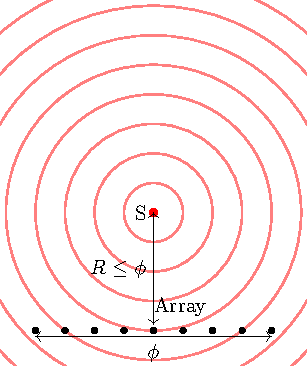
\includegraphics[width=\textwidth]{NearField.pdf}
        \caption{Near-Field Case}
        \label{fig:y equals x}
    \end{subfigure}
    \hfill
    \begin{subfigure}[b]{0.45\textwidth}
        \centering
        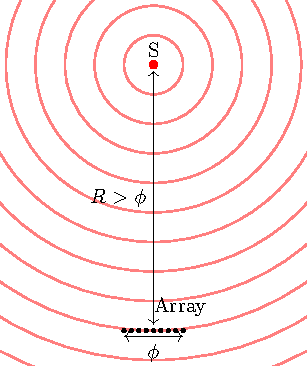
\includegraphics[width=\textwidth]{FarField.pdf}
        \caption{Far-field Case}
        \label{fig:three sin x}
    \end{subfigure}
    \caption{Three simple graphs}
    \label{fig:three graphs}
\end{figure}



%\begin{figure}
%    \centering
%%    \includegraphics[width=0.25\textwidth]{mesh}
%    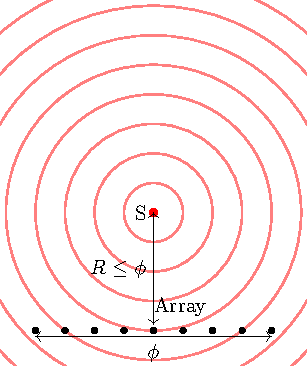
\includegraphics[]{NearField.pdf}
%    \caption{a nice plot}
%    \label{fig:mesh1}
%\end{figure}



\appendix
% \chapter{Appendix}
\clearpage

\section{Declaration of Authorship} \label{Declaration of Authorship}
We hereby certify that the thesis we are submitting is entirely our own original work except where otherwise indicated.
We are aware of the University's regulations concerning plagiarism, including those regulations concerning disciplinary actions that may result from plagiarism.
Any use of the works of any other author, in any form, is properly acknowledged at their point of use.

\bigskip
\textbf{Location, Date} \\
Rapperswil, 24. January 2024

\vspace{1.2cm}
\begin{tabular}{@{}p{0.1cm}p{6cm}p{0.6cm}p{6cm}@{}}
	 & \hrulefill          &  & \hrulefill   \\ \\[-0.7em]
	 & Florian Baumgartner &  & Alain Keller \\
\end{tabular}


\includegraphics[width=4.8cm, align=t, smash=br, hshift=0.9cm, vshift=2.55cm]{appendix/Signature_Florian_Baumgartner.pdf}
% \includegraphics[width=3.6cm, align=t, smash=br, hshift=8.25cm, vshift=2.2cm]{appendix/Signature_Alain_Keller.pdf}
\todo{Add Alain's signature here}
\newpage

\section{Data Archive} \label{Data Archive}
All created files and documents of this project are publicly available on GitHub. An institution called \textbf{PA-OST-2023} (\url{https://github.com/PA-OST-2023}) has been founded which contains repositories for each individual part of the project.
A quick description of the repositories including the associated web link is listed below:

\subsubsection{heron-administration} \vspace{-0.2cm}
\begin{description}
	\item[Description:] This repository contains all confidential information of the project.\vspace{-0.25cm}
	\item[URL:] \url{https://github.com/PA-OST-2023/heron-administration}\vspace{-0.25cm}
	\item[Type:] Private\vspace{-0.25cm}
\end{description}

\subsubsection{heron-literature} \vspace{-0.2cm}
\begin{description}
	\item[Description:] This repository contains all literature used in this project.\vspace{-0.25cm}
	\item[URL:] \url{https://github.com/PA-OST-2023/heron-literature}\vspace{-0.25cm}
	\item[Type:] Private\vspace{-0.25cm}
\end{description}

\subsubsection{heron-documentation} \vspace{-0.2cm}
\begin{description}
	\hfuzz=35.0pt
	\item[Description:] This repository contains this document.\vspace{-0.25cm}
	\item[URL:] \url{https://github.com/PA-OST-2023/heron-documentation}\vspace{-0.25cm}
	\item[Type:] Public\vspace{-0.25cm}
\end{description}

\subsubsection{heron-hardware} \vspace{-0.2cm}
\begin{description}
	\item[Description:] This repository contains hardware related documents (Schematics, PCB).\vspace{-0.25cm}
	\item[URL:] \url{https://github.com/PA-OST-2023/heron-hardware}\vspace{-0.25cm}
	\item[Type:] Public\vspace{-0.25cm}
\end{description}

\subsubsection{heron-firmware} \vspace{-0.2cm}
\begin{description}
	\item[Description:] This repository contains firmware source code written in C++.\vspace{-0.25cm}
	\item[URL:] \url{https://github.com/PA-OST-2023/heron-firmware}\vspace{-0.25cm}
	\item[Type:] Public\vspace{-0.25cm}
\end{description}

\subsubsection{heron-simulator} \vspace{-0.2cm}
\begin{description}
	\item[Description:] This repository contains the simulator source code written in Python.\vspace{-0.25cm}
	\item[URL:] \url{https://github.com/PA-OST-2023/heron-simulator}\vspace{-0.25cm}
	\item[Type:] Public\vspace{-0.25cm}
\end{description}

\subsubsection{heron-application} \vspace{-0.2cm}
\begin{description}
	\item[Description:] This repository contains the application source code written in Python.\vspace{-0.25cm}
	\item[URL:] \url{https://github.com/PA-OST-2023/heron-application}\vspace{-0.25cm}
	\item[Type:] Public\vspace{-0.25cm}
\end{description}

\subsubsection{heron-mechanical} \vspace{-0.2cm}
\begin{description}
	\item[Description:] This repository contains mechanical related documents (CAD-Files).\vspace{-0.25cm}
	\item[URL:] \url{https://github.com/PA-OST-2023/heron-mechanical}\vspace{-0.25cm}
	\item[Type:] Public\vspace{-0.25cm}
\end{description}

\subsubsection{heron-bastelstube} \vspace{-0.2cm}
\begin{description}
	\item[Description:] This repository contains temporary and experimental files.\vspace{-0.25cm}
	\item[URL:] \url{https://github.com/PA-OST-2023/heron-bastelstube}\vspace{-0.25cm}
	\item[Type:] Private\vspace{-0.25cm}
\end{description}
\newpage

% Definition of Task
% Datasheet of MEMS microphone
% Schematics of Microphone Boards
% PCB Design of Microphone Boards
% BOM of Microphone Boards
% Schematics of Acquisition-System
% PCB Design of Acquisition-System
% BOM of Acquisition-System
% Schematics of Mainboard
% PCB Design of Mainboard
% BOM of Mainboard
% Schematics of Microphone-Arms
% PCB Design of Microphone-Arms
% BOM of Microphone-Arms
% Schematics of Angle-Sensor
% PCB Design of Angle-Sensor
% BOM of Angle-Sensor
% Mechanical Drawings of each component

\backmatter
\bibliography{sections/bibliography.bib}
\bibliographystyle{plain}
\typeout{}

\end{document}